% !TeX root = ../main.tex

\xchapter{可配置计算核心（Core）与全系统同步机制}{Configurable Core and System Synchronization}

第三章已给出模拟器的总体架构、IR 解析流程以及 NoC/DRAM 的接口抽象（网络接口、存储接口）。本章在此基础上展开\textbf{执行层}的设计。具体包括：单核如何按依赖驱动推进、如何通过上述接口发起请求与接收响应。多核并发下核间通信与 NoC/DRAM 资源争用如何体现、如何保证因果一致与可复现。最后说明全局周期与多时钟域如何同步，从而完成从“接口契约”到“可运行系统”的闭环。

\xsection{高通用性计算核心建模}{General-purpose Core Modeling}

\xsubsection{建模目标与抽象边界}{Modeling Goals}

多核 NPU 端到端性能受计算、通信与存储共同影响。为在系统级研究中兼顾通用性与可解释性，本文以调度器 IR 中的“工作负载”为最小执行单元，对核心执行过程进行依赖驱动建模。核心在满足输入依赖后进入计算，计算完成后将输出写入本地 SRAM 并供其他核心拉取或写回 DRAM。该抽象能够覆盖 MAC 密集算子（卷积、全连接）与向量/逐元素算子（池化、激活等），并保留“等待依赖到齐”“注入队列满导致背压”“写回 DRAM 拖尾”等关键瓶颈形成机制，便于在第五章对端到端周期做阶段分解与归因。

从方法论上，以工作负载而非单条指令为粒度建模，是在“可解释性”与“仿真成本”之间的折中。指令级模拟能刻画更细的流水与调度行为，但多核、多 workload 场景下事件规模大，难以快速扫描配置。工作负载级抽象将调度器已决策的依赖与数据量作为输入，使端到端周期可归结为“计算—加载—写回”等阶段的叠加。由此便于回答“瓶颈在计算、通信还是存储”“增加某类资源能否线性缩短时间”等系统级问题，为架构探索与调度—硬件协同研究提供可操作的评估界面。

单核在模拟中的职责边界为：维护当前工作负载队列与当前下标、按状态机推进、在“加载”阶段向 NoC/DRAM 发起读请求并消费到达的读响应、在“写回”阶段向 DRAM 发起写请求并等待写响应、响应他核对本核 SRAM 中已就绪数据的读请求。核心不直接调用 NoC/DRAM 的注入或发请求接口，而是将待发送的报文放入内部发送队列，由模拟引擎在每周期推进后统一从各核收集报文并注入网络或存储。到达的包由引擎按节点或目的核投递到各核的接收入口，核心在下一周期推进开头先处理本周期到达的报文。由此保证“同一周期内先推进核心、再收集发送、再推进 NoC/DRAM、再投递”的因果顺序。

\xsubsection{状态机设计}{State Machine}

本文将单核执行抽象为五态状态机：空闲、加载、计算、写回、完成。状态转移在单周期推进内按当前状态分支执行。

\textbf{空闲。} 若当前工作负载下标已达队列末尾，则转入“完成”并结束该核。否则取当前工作负载，根据其输入依赖中所有数据源的传输标识填入“待加载集合”。若待加载集合为空（无输入依赖），则直接转入“计算”并设置剩余计算周期。否则转入“加载”，等待依赖到齐。

\textbf{加载。} 每周期尝试发起取数请求。对尚未请求过的传输标识，若已在本地 SRAM 且已就绪则从待加载集合移除。否则若来源为“他核”则构造发往该核的读请求，若来源为 DRAM 则构造发往 DRAM 的读请求，放入发送队列（若队列已满则统计“因 NoC 背压停滞”的周期数并本周期不再注入）。当“所有缓冲已加载”（即待加载集合为空）时，转入“计算”并设置剩余计算周期。

\textbf{计算。} 每周期剩余计算周期减一。减至 0 时将当前工作负载的输出在 SRAM 中分配并标记为就绪（引用计数由 IR 后处理给出），并释放已消费的输入缓冲（对输入传输标识执行引用释放）。若存在输出目的为 DRAM，则转入“写回”并初始化待写回队列。否则当前工作负载完成，当前下标自增，回到“空闲”。

\textbf{写回。} 每周期按 SRAM 读带宽从当前待写回块读取数据，凑满可发送的写请求后构造写请求（目的为 DRAM）放入发送队列，并将该传输标识加入“待写回完成集合”。当“所有写请求已发出且写响应均已收回”时，当前工作负载完成，回到“空闲”。

\textbf{完成。} 该核不再参与推进。

每周期推进内，在状态分支之前先执行以下操作。处理本周期投递来的包。将 NoC/DRAM 读响应数据按写带宽写入 SRAM 并标记就绪。对他核发来的读请求，若本核 SRAM 已就绪则回复读响应，否则继续挂起。图\ref{fig:c4_fsm} 给出状态机示意。
\vspace{-0.8em}
% 图片由 thesis/Figures/c4_core_fsm.drawio 导出为 PDF 后使用。
\begin{figure}[htbp]
  \centering
  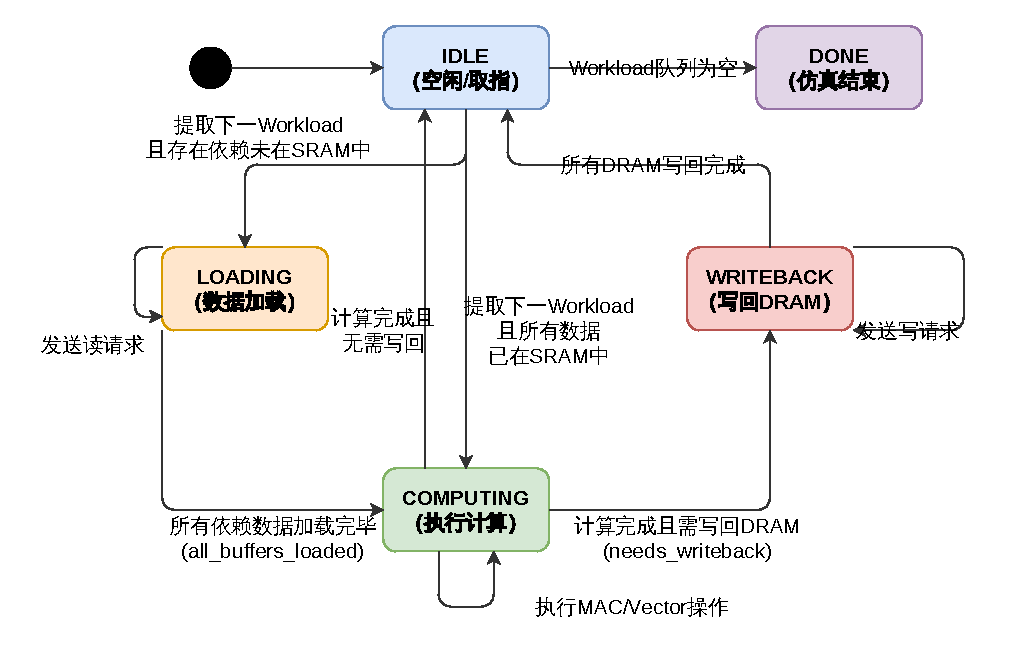
\includegraphics[width=0.85\linewidth]{Figures/c4_core_fsm.pdf}
  \caption{核心状态机示意}
  \label{fig:c4_fsm}
\end{figure}
\vspace{-0.6em}

% \begin{lstlisting}[language={},caption={Mermaid 源码：Core 状态机},label={lst:mermaid:fsm}]
% stateDiagram-v2
%   [*] --> IDLE
%   IDLE --> LOADING: pending_loads 非空
%   IDLE --> COMPUTING: pending_loads 为空
%   IDLE --> DONE: 无剩余 workload
%   LOADING --> COMPUTING: all_buffers_loaded
%   COMPUTING --> WRITEBACK: 存在 DRAM 写回
%   COMPUTING --> IDLE: 无写回，workload 完成
%   WRITEBACK --> IDLE: all_writebacks_complete
% \end{lstlisting}

\xsubsection{计算资源与参数化模型}{Parameterized Compute Model}

核心计算能力由配置中的“MAC 单元数”与“向量单元数”刻画，分别用于 MAC 密集算子与向量/逐元素算子的周期估算。周期估算逻辑为：若启用解析周期且 IR 中提供了该值，则直接采用。否则对卷积/全连接按“总 MAC 数除以 MAC 单元数”上取整，对池化/逐元素/点对点按“输出元素数除以向量单元数”上取整。该模型强调可配置性与可对比性。一方面与调度器 IR 中的解析周期或算子形态对接，保证单 workload 计算时长在给定配置下可复现。另一方面将 MAC/向量单元数作为可调参数，便于在尚未流片或缺乏多组硬件实测时进行敏感性分析。例如在第五章中扫描 MAC 单元数等参数，观察“计算资源提升的边际收益递减”与“瓶颈从计算迁移到通信/存储”等现象，为“计算墙—通信墙—存储墙”的定量刻画提供依据。

\xsubsection{本地 SRAM 建模与生命周期}{Local SRAM Modeling}

本地 SRAM 按“容量（字节）+ 读/写带宽（字节每周期）”建模，内部以传输标识为键维护条目，每项包含大小、数据类型（输入特征/权重/输出特征）、是否已就绪、引用计数（仍在引用该数据的消费者数）。分配时在容量允许下登记条目并累加已用容量。标记就绪将对应条目置为可消费。释放引用将引用计数减一，减至 0 时回收容量。这样，多消费者共享同一输出时，该输出在 SRAM 中保留至最后一个消费者释放引用，与第二章所述 IR 语义及解析器的引用计数后处理一致。

\textbf{SRAM 拉取策略。} 第四章后文所述核间与 DRAM 的拉取式数据流，在“网络与存储接口”层面体现为消费者发起读请求、数据以读响应形式到达。在\textbf{本地 SRAM}层面，本文采用与之衔接的\textbf{到达后再占位、就绪后才可消费}的策略，可概括为三点。（1）\textbf{请求不等于已入 SRAM}。核心在“加载”阶段发出读请求，仅表示向对端或 DRAM 索要数据，并不在本地预先为整块数据预留可消费条目。数据只有在读响应到达并被核心处理之后，才进入本地 SRAM 管理流程。（2）\textbf{响应到达后的分配与写入}。读响应到达时，仿真器先按当前 workload 对该输入的引用关系确定引用计数，并尝试为对应传输标识执行容量分配。若当前剩余容量不足，则将该响应暂存于重试队列，在后续周期中随其他数据释放或配置变化再次尝试分配，避免因瞬时峰值误判为永久失败。分配成功后，将本次加载的字节数记入“待写入 SRAM 的剩余量”，并在每个周期按有效写带宽（见下）消耗剩余量。当某传输标识对应的剩余量减至零时，将该条目标记为就绪，并从“待加载集合”中移除。由此，\textbf{网络/存储侧完成传输}与\textbf{片上写入带宽填满本地 SRAM 并置就绪}在时间上可分步刻画，便于区分“远端延迟”与“片上写口瓶颈”。（3）\textbf{核间读对生产者 SRAM 的拉取}。消费者向生产者发起的读请求，仅在生产者本地 SRAM 中该传输标识已就绪时立即回复读响应。否则请求挂起，待生产者侧计算完成并将输出写入本地 SRAM 并标记就绪后再回复。生产者侧在成功向消费者发送读响应时，按语义对相应条目做引用释放。这与（1）（2）共同构成“谁消费、谁拉取、何时在本地变为可消费”的闭环。

\textbf{带宽与类型分档。} 有效写带宽与有效读带宽可根据当前 workload 类型在 PE 与 VP 两档配置间选取（例如卷积、全连接走 PE 档带宽，其余走 VP 档），与配置中统一写带宽字段并存。若将某档带宽配置为 0，则仿真器退化为“当拍内完成整块逻辑写入并标记就绪”，用于与带宽受限模式对照。每周期更新 SRAM 统计中的峰值占用，供第五章分析 SRAM 占用与映射可行性。峰值占用与引用计数语义的结合，使得“某调度在给定 SRAM 容量下是否可行”“若缩小容量何处会成为瓶颈”等问题可在仿真中直接观测，为映射与缓冲配置的可行性研究提供定量支撑。

\xsubsection{统计输出与可观测性}{Observables and Statistical Output}

执行层在每核、每周期上的行为最终体现为可导出的统计与踪迹，这些输出是连接“设计”与“分析”的桥梁。仿真结束后，每核可汇总得到在空闲、加载、计算、写回及因 NoC 背压停滞各阶段的周期数，以及完成的 workload 数、加载/写回的数据量、SRAM 峰值占用等。若开启状态追踪，还可按周期记录各核的状态转移序列（如从加载转入计算、从计算转入写回等），进而生成按核、按时间排列的阶段甘特图。上述统计与踪迹不改变仿真语义，但为端到端周期的阶段分解、瓶颈归因以及“热点核”识别提供了统一口径。第五章将基于这些可观测量，对真实负载进行“计算—访存—NoC 背压”的占比分解，并对多核场景下的 workload 时间线进行可视化，从而在系统级回答“时间花在哪里”“哪些核或哪些阶段主导了总周期”等问题。

\xsection{NoC 与 DRAM 子系统的集成机制}{Integration of NoC and DRAM}

第三章定义的网络接口与存储接口为执行层提供了统一的注入、推进与响应提取能力。本节说明模拟引擎与核心如何在使用这两类接口的前提下，将核间通信与 DRAM 访问纳入统一模型。

\textbf{拉取式数据流与报文统一。} 核间数据采用拉取式（pull-based）数据流。消费者核心在“加载”阶段根据缓冲需求中的来源列表，向生产者核心（来源类型为“他核”时按源核 ID）或 DRAM（来源类型为 DRAM 时）发起读请求。生产者核心在处理到达报文时收到读请求。若本地 SRAM 中该传输标识已就绪，则构造读响应放入发送队列。否则将请求加入“待回复的远端读请求”列表，在后续周期中当数据就绪且发送队列未满时再回复。DRAM 读请求由引擎根据地址分配器填入物理地址后交给存储接口。写请求同样目的为 DRAM，由引擎注入 DRAM，DRAM 完成后再以写响应经引擎投递回核心，核心在处理到达报文时从“待写回完成集合”移除对应传输标识。所有报文均使用统一的报文结构（类型、源/目的、传输标识、数据大小、地址等），便于 NoC 与 DRAM 共用同一抽象\cite{jiang2013booksim,luo2023ramulator2}。

从研究角度，拉取式数据流与统一报文使“核间读请求—响应”与“DRAM 读/写请求—响应”在模拟中的处理路径一致，便于在对比实验中有意隔离变量。例如比较“仅 DRAM 依赖”与“含核间依赖”的负载时，可明确区分 NoC 流量与 DRAM 流量的贡献，为第五章中微基准设计与后端差异分析提供清晰的语义基础。

\textbf{引擎侧收集与投递。} 在单周期推进中，各核心推进后，引擎遍历各核的待发送报文。若目的为 DRAM，则用地址分配器填入物理地址，再根据拓扑决定是经 NoC 发往 DRAM 控制器节点还是直接交给存储接口。若目的为他核，则必要时将源/目的转为 NoC 节点 ID 后注入网络接口。投递 NoC 包时按节点取回本周期到达的包并交给对应核心的接收入口（或交给 DRAM 控制器节点再转发给存储接口）。投递 DRAM 响应时从存储接口取回本周期完成的响应，根据目的投递给对应核心（若 DRAM 挂在 NoC 上，则响应先经 NoC 再在下一周期投递）。拓扑负责核心 ID 与 NoC 节点 ID 的映射、DRAM 控制器节点 ID 以及多控制器时的路由策略，从而支持“仅计算核挂 NoC”与“NoC 上挂 DRAM 控制器”两种部署方式。

\textbf{背压与队列约束。} 核心侧发送队列容量由网络接口配置限定。当队列满时，新发出的请求无法入队，本周期统计“因 NoC 背压停滞”的周期数，请求在下一周期重试。NoC 侧“是否可注入”在 BookSim2 封装中反映注入缓冲是否满，引擎可将无法注入的 DRAM 响应缓存在待注入队列并在后续周期重试注入，从而形成背压传递，使端到端周期能够反映拥塞与排队效应。

\xsubsection{多核并发与资源争用}{Multi-core Concurrency and Resource Contention}

对于数据流驱动的多核 NPU，同一全局周期内多核并行推进，核间通信与共享资源的争用会直接影响端到端周期与瓶颈分布，仅讨论单核状态机不足以刻画系统行为。本小节说明多核并发在模拟中的体现、可能出现的竟态与争用现象，以及本文如何通过确定的推进顺序与资源建模来刻画并复现这些效应。

\textbf{多核并发的体现。} 在单周期推进中，引擎先对各核心依次执行一次推进，再从\textbf{所有}核心收集本周期发出的包并注入 NoC/DRAM。因此，每一全局周期内，多个核心可能同时处于“加载”（向不同生产者或 DRAM 发起读请求）、“计算”或“写回”。它们产生的请求在同一周期或相邻周期内集中进入 NoC 与 DRAM 的队列，形成对共享链路与存储资源的并发访问。依赖关系由 IR 中的传输标识与各核的“待加载集合”保证。消费者只有在收到对应读响应并标记就绪后才会离开“加载”，但“何时收到”取决于 NoC 的投递延迟与 DRAM 的排队与调度，二者均受多核并发流量影响。

\textbf{竟态与争用现象。} （1）\textbf{NoC 争用}。多核同时向 NoC 注入时，同一链路或路由器上的多包需仲裁与排队。BookSim2 的虚拟通道分配、交换分配与路由延迟会随流量增大而放大尾延迟，部分核心的响应包可能因拥塞晚于“理想延迟”到达，从而拉长其“加载”阶段并统计到更多“因 NoC 背压停滞”周期。（2）\textbf{DRAM 争用}。多核的读/写请求进入同一 DRAM 控制器后，Bank/行缓冲与调度器（如 FR-FCFS）会引入排队与行冲突。Ramulator2 按时序与调度策略推进，同一周期内完成的响应数受通道与 Bank 并行度限制，部分请求的响应会延后完成，体现为消费者核心在“加载”或“写回”阶段等待更久。（3）\textbf{生产者侧背压}。当消费者向生产者发起读请求时，生产者需在数据就绪后回复读响应。若生产者本周期发送队列已满（因其他响应或本核写回占用），则无法注入该响应，请求在“待回复的远端读请求”中挂起，消费者端待加载集合无法清空，形成跨核的背压链。上述现象在真实多核数据流执行中均存在，本文通过“多核每周期同时推进 + 统一收集注入 + NoC/DRAM 周期级建模”将其显式刻画为可观测的周期与阶段占比。

\textbf{确定性顺序与可复现性。} 模拟器内部不引入随机调度。同一周期内核心按数组下标顺序推进，收集报文按相同顺序遍历并注入，NoC/DRAM 的仲裁与调度由配置与请求到达顺序确定。因此，多核并发下的“谁先被服务”由确定的规则与数据依赖决定，不存在未定义的竟态。同一配置与同一 IR 下，总周期与各核各阶段占比可完全复现。争用与排队体现在“同一资源被多核同时使用时，部分请求被延迟”的客观结果上，而非模拟器实现的不确定性。

\textbf{死锁与核间同步。} 在拉取式数据流与有限发送队列的约束下，多核推进可能陷入\textbf{死锁}。若干核心均在“加载”或“写回”阶段等待来自他核或 DRAM 的响应，而对方因自身队列已满或尚未产生数据无法注入响应，形成相互等待、全局不再推进的局面。死锁的成因可从两方面理解。（1）\textbf{依赖与资源环}。若调度 IR 中存在跨核的依赖环（例如核心 A 的某 workload 依赖核心 B 的输出，核心 B 的某 workload 又依赖核心 A 的输出，且二者在时间上重叠或请求顺序导致互相阻塞），则在没有额外同步或请求排序约束时，可能出现“A 等 B、B 等 A”的循环等待。IR 本身描述的是数据依赖关系，调度器在生成 IR 时通常假定执行按某种顺序或缓冲容量充足，但并未在 IR 中显式编码“防死锁”的调度约束，因此 IR 在语义上并不保证无环或可运行性。（2）\textbf{队列与背压的级联}。当生产者核心的发送队列已满时，无法向消费者回复读响应，消费者会一直停留在“加载”并可能持续发起重试。若 NoC 或 DRAM 的注入侧也因背压无法接受新包，则请求与响应在多个节点上形成阻塞链，在极端情况下可能演变为系统级停滞。

当前模拟器\textbf{未实现}显式的死锁检测、避免或恢复机制。既无对 IR 依赖图的静态环检测，也无运行时超时或心跳判定，亦无在注入顺序、虚拟通道分配或请求优先级上的保守策略以在理论上保证活性。因此，在部分多核负载或特定配置（如发送队列较小、NoC 缓冲较紧）下，仿真可能在实际运行中观察到“总周期不再增长、各核状态不再变化”的死锁现象。这既可能暴露调度或 IR 中存在的依赖环或资源估计不足，也提示模拟器在后续改进中可引入的增强方向。例如在 IR 解析后对跨核依赖做有向图环检测并给出警告。在引擎侧对“连续若干周期无任何核心状态变化”做超时判定并终止或报告。或在请求注入时采用保守排序（如按依赖拓扑序、或按核 ID 约束请求发出顺序）以在给定假设下避免部分死锁。上述讨论旨在将死锁与核间同步作为多核数据流模拟中的固有议题加以明确，为理解实验现象与后续机制扩展提供概念基础。

图\ref{fig:c4_concurrency} 给出多核并发下请求汇聚与资源争用的示意。多核在各自 LOADING/WRITEBACK 中产生的请求经引擎统一注入 NoC/DRAM，NoC 与 DRAM 在共享队列与仲裁下推进，响应再经投递回到各核，部分核心因排队或背压而在 LOADING/WRITEBACK 上停留更久，从而在端到端周期与阶段分解中体现核间通信与共享资源的影响。值得指出的是，争用与背压在模拟中并不依赖随机调度，而是由确定的推进顺序与请求到达顺序产生。因此“因 NoC 背压停滞”的周期数、各核在加载/写回阶段的占比等均可稳定复现，并可作为第五章中多核瓶颈分解与热点核分析的数据基础。当负载从单核扩展到多核时，非零的 NoC 背压占比与各核阶段分布的差异，恰好用于回答“通信是否成为新瓶颈”“哪些核受争用影响最大”等设计问题。

% 图片由 scripts/plot_c4_concurrency.py 生成，或由 thesis/figures/c4_concurrency.drawio 导出。
\begin{figure}[htbp]
  \centering
  
\includegraphics[width=\linewidth]{figures/c4_concurrency.pdf}
  \caption{多核并发下请求汇聚与 NoC/DRAM 争用示意}
  \label{fig:c4_concurrency}
\end{figure}

\xsection{全局事件驱动与跨时钟域同步}{Event-driven Scheduling and Cross-clock-domain Synchronization}

模拟器以全局周期为唯一时间基准。全局周期计数器在每次“单周期推进”时递增一次，同一推进内各模块的顺序固定为“先核心、再收集注入、再 NoC/DRAM 推进、再投递”，从而保证请求先于响应、响应在后续周期被核心消费的因果关系。然而，当核心、NoC 与 DRAM 控制器运行在不同时钟域时，若仍按“每全局周期各子系统均推进一周期”的假设建模，既无法反映真实频率差异，也可能在因果顺序与周期统计上产生歧义。本节先说明跨时钟域模拟面临的主要问题，再介绍本文的设计与实现，最后用图示归纳多速率推进的时序关系及可达效果。

\xsubsection{跨时钟域模拟面临的问题}{Challenges in Cross-clock-domain Simulation}

\textbf{（1）时间基准不统一。} 真实芯片中，计算核心、NoC 路由器与 DRAM 控制器往往由不同 PLL 或时钟域驱动，三者频率可能为 1\,GHz / 500\,MHz / 266\,MHz 等不同组合。若模拟器仅使用“单一周期计数器”且每拍让所有子系统各推进一周期，则等价于假设三者同频，无法区分“DRAM 控制器更慢”带来的排队与带宽折减。若改为为每个子系统维护独立时钟并异步推进，则事件顺序与“谁先谁后”的判定会变得复杂，且请求在“核心周期 $t$”发出、响应在“DRAM 周期 $t'$”完成时，需要明确 $t$ 与 $t'$ 的对应关系才能正确投递响应并统计端到端延迟。

\textbf{（2）因果一致与响应可见性。} 请求在某一时刻注入 NoC 或 DRAM 后，响应应在“该子系统已处理该请求并完成传输/访问”之后才对核心可见。若子系统的“内部周期”与“全局周期”不一致，则必须约定响应何时被认为“已完成”，是以全局周期为刻度还是以子系统自身周期为刻度。若约定不当，可能出现“响应在逻辑上早于请求被处理”的因果错误，或同一全局周期内事件顺序依赖实现细节而难以复现。

\textbf{（3）周期统计与带宽语义。} 端到端“总周期”通常以核心或系统主时钟为统计口径。当 DRAM 以较低频率运行时，其“每 DRAM 周期处理能力”不变，但“每全局周期平均处理能力”会按频率比下降。模拟器需要在保持因果正确的前提下，让 DRAM 的等效带宽与“每全局周期可完成的请求数”随时钟比合理变化，以便扫描时钟比时观察到“内存变慢→端到端周期增加”的预期趋势。

\xsubsection{本文的设计：全局周期与多速率推进}{Design: Global Cycle and Multi-rate Ticking}

本文采用“单一全局周期 + 多速率推进”的策略，在不动引擎调用顺序的前提下，让 NoC 与 DRAM 的“等效频率”可配置。

\textbf{统一时间基准。} 以全局周期计数器为唯一时间轴，所有“何时发生”的判定均以该周期为刻度。核心每全局周期推进一次。NoC 与 DRAM 的“推进”由引擎在每全局周期调用一次，但接口内部可根据“时钟比”决定本全局周期内子系统是否推进、以及推进几次。

\textbf{时钟比语义。} 配置项“NoC 时钟比”与“DRAM 时钟比”的约定为：时钟比 = 核心频率 / 子系统频率。因此时钟比 = 1 表示子系统与核心同频（每全局周期推进一周期）。时钟比 = 2 表示子系统以核心一半频率运行（每 2 个全局周期推进 1 周期）。时钟比 < 1 表示子系统频率高于核心（每全局周期可能推进多次，本项目通过累加器的累加与扣减实现）。这样，配置与真实“核心 1\,GHz、DRAM 500\,MHz”的对应关系为 DRAM 时钟比 = 2，便于与数据手册或 RTL 时钟设定对齐。

\textbf{累加器实现。} BookSim2 封装与 Ramulator2 封装内维护浮点累加器。每次被引擎调用时（即每全局周期一次）累加 1。当累加值不小于时钟比时，执行一次内部网络或存储的推进，并扣减时钟比（若时钟比大于 1，可用循环保证不漏推进）。因此，在任意一段全局周期数 $G$ 内，NoC/DRAM 的“等效推进次数”为 $G/\text{时钟比}$（取整由累加器自然体现）。既满足因果（请求先进入队列，随后仅在子系统推进时被处理），又使响应完成时间随时钟比增大而延后，从而在端到端周期上体现“内存更慢”的效果。

\xsubsection{时序示意与效果}{Timeline Illustration and Effects}

图\ref{fig:c4_cdc_timeline} 与表\ref{tab:c4_cdc_timeline} 给出在 DRAM 时钟比为 2 时，连续若干全局周期内核心、NoC 与 DRAM 的推进关系。核心每全局周期推进一次。DRAM 仅在累加值达到时钟比时推进，因此第 0、2、4、6 拍才各推进一次，等效于“每 2 个全局周期 1 个 DRAM 周期”。请求在某一全局周期注入 DRAM 后，需等待 DRAM 内部经过若干次推进才会在“取回响应”时返回。由于 DRAM 推进频率降低，同一请求的“从注入到响应可见”的全局周期数会随时钟比增大而增加，从而在总周期与瓶颈分析中体现跨时钟域影响。

\begin{figure}[htbp]
  \centering
  \fbox{\parbox{0.92\linewidth}{%
    \small
    \vspace{0.4em}
    \textbf{全局周期（唯一时间轴）：} $g=0$\quad 1\quad 2\quad 3\quad 4\quad 5\quad 6\quad …\\
    \vspace{0.3em}
    \textbf{核心 / NoC（时钟比=1）：} 每拍推进一次。\\
    \textbf{DRAM（时钟比=2）：} 仅在累加值$\ge$2 时推进，即 $g=0,2,4,6,\ldots$ 各推进 1 次。等效“每 2 全局周期 1 DRAM 周期”。
    \vspace{0.5em}\\
    \hrule
    \vspace{0.4em}
    累加器变化示例：$g=0$ 时 +1$\to$1，1$<$2 不推进。$g=1$ 时 +1$\to$2，2$\ge$2 推进并 -2$\to$0。依此类推。
    \vspace{0.6em}
  }}
  \caption{跨时钟域多速率推进时序示意（DRAM 时钟比=2 时，每 2 个全局周期 DRAM 推进 1 次）}
  \label{fig:c4_cdc_timeline}
\end{figure}

\begin{table}[htbp]
  \centering
  \caption{多速率推进示例（DRAM 时钟比=2）}
  \label{tab:c4_cdc_timeline}
  \begin{tabular}{c|ccccccc|l}
    \hline
    全局周期 $g$ & 0 & 1 & 2 & 3 & 4 & 5 & 6 & \ldots \\
    \hline
    Core 推进 & $\checkmark$ & $\checkmark$ & $\checkmark$ & $\checkmark$ & $\checkmark$ & $\checkmark$ & $\checkmark$ & 每拍一次 \\
    NoC 推进（ratio=1） & $\checkmark$ & $\checkmark$ & $\checkmark$ & $\checkmark$ & $\checkmark$ & $\checkmark$ & $\checkmark$ & 每拍一次 \\
    DRAM 推进（ratio=2） & $\checkmark$ & -- & $\checkmark$ & -- & $\checkmark$ & -- & $\checkmark$ & 每 2 拍一次 \\
    累加器（DRAM） & 1 & 2$\to$0 & 1 & 2$\to$0 & 1 & 2$\to$0 & 1 & 累加至 $\ge$2 则推进并扣减 \\
    \hline
  \end{tabular}
\end{table}

% 清单\ref{lst:mermaid:cdc} 用 Mermaid 给出“每全局周期：先核心、再收集注入、再 NoC/DRAM 推进、再投递”的流程，以及 NoC/DRAM 内部“累加器累加与条件推进”的抽象逻辑，便于复现与扩展。

% \begin{lstlisting}[language={},caption={Mermaid 源码：跨时钟域 tick 流程},label={lst:mermaid:cdc}]
% flowchart LR
%   subgraph global[" 每全局周期 "]
%     A[Core tick] --> B[collect inject]
%     B --> C[NoC/DRAM tick]
%     C --> D[deliver]
%   end
%   subgraph noc_dram[" NoC/DRAM 内部 "]
%     E[tick_accum += 1]
%     E --> F{tick_accum >= ratio?}
%     F -->|是| G[内部 tick, tick_accum -= ratio]
%     F -->|否| H[本拍不推进]
%   end
% \end{lstlisting}

\textbf{效果小结。} （1）\textbf{因果一致}。请求在某一全局周期被提交或注入后，仅在后续全局周期中、当子系统内部已推进并完成该请求时，响应才会在“取回响应”或“按节点取回包”时出现并投递给核心，不会出现“响应早于请求”。（2）\textbf{可复现}。同一配置与同一 IR 下，总周期与各阶段占比由确定的时钟比与累加器逻辑决定，无随机性或实现依赖。（3）\textbf{可配置与可探索}。通过将 DRAM（或 NoC）的时钟比设为大于 1，即可在不改动核心与引擎代码的前提下刻画“内存/网络相对更慢”的场景，便于在第五章进行参数扫描与“存储墙/通信墙”敏感性分析。

\xsection{模拟器支撑的研究与探索视角}{Research and Exploration Enabled by the Simulator}

前文从执行层设计出发，给出了单核状态机、NoC/DRAM 集成与跨时钟域同步的具体实现。本节从“可做什么研究”的角度，归纳上述设计所支撑的几类系统级研究与探索，并与第五章的验证与实验形成呼应。这样做的目的，一是明确本模拟器在学术与工程中的定位。它不仅是实现层面的技术闭环，更是面向多核 NPU 架构与调度—硬件协同研究的评估平台。二是为读者提供从“机制”到“应用”的过渡，使后续章节中的微基准验证、瓶颈分解与设计空间探索在动机上有据可依。

\textbf{瓶颈归因与阶段分解。} 端到端执行时间由计算、核间通信与片外访存共同决定。但在缺乏周期级可观测量的情况下，难以回答“时间主要花在计算、等待数据加载还是写回 DRAM”多核扩展后通信是否取代计算成为主导瓶颈”等问题。本模拟器在每核上统计加载、计算、写回及因 NoC 背压停滞的周期数，并可选择性地导出按周期的状态转移踪迹，从而将总周期分解为“计算占用”“访存相关等待”与“NoC 背压”等可解释分量。该分解口径具有明确的语义（与状态机阶段一一对应）且可复现，适用于对调度器生成的 IR 进行事后分析。第五章将基于该口径对 ResNet 等真实负载进行占比分解，得到“计算约占多少、访存约占多少”的定量结果，为调度优化与资源调配提供依据。在多核场景下，非零的 NoC 背压占比与各核阶段分布的差异还可用于识别“热点核”与通信密集时段，与第五章中的热点核与 workload 甘特图分析相对应。

\textbf{微基准与因果验证。} 在将模拟器用于大规模负载或设计空间探索之前，需要先确认其基本行为与预期一致。例如核间依赖是否被正确遵守、DRAM 请求与响应是否形成闭环、不同 NoC/DRAM 后端在计算阶段是否一致而在访存阶段是否体现时序差异。这些问题的回答依赖于可控的微基准实验，例如双核点对点依赖（生产者—消费者）、单核仅 DRAM 依赖（无核间通信）等。通过对比“消费者是否在生产者完成后才结束加载”“NoC 包数是否与预期一致”“simple 与 full 后端在总周期与各阶段时长上的差异是否集中在访存”等，验证因果一致性与后端差异的隔离性。第五章的 MB-1 与 MB-2 即在此思路下设计，并为后续与 ZeBu 硬件模拟的精度对比奠定基础。从本章视角看，这些实验所依赖的“统一推进顺序、可导出的状态时间线、按阶段可比的周期数”均来自前文所述执行层与统计输出设计。

\textbf{设计空间探索与参数敏感性。} 多核 NPU 的设计空间涉及核心计算能力、片上缓存容量、NoC 拓扑与缓冲、DRAM 通道与时序等多维参数。在流片前或缺乏多组硬件实测时，仿真成为探索该空间的主要手段。本模拟器将核心 MAC/向量单元数、SRAM 容量与带宽、NoC 与 DRAM 的后端与时钟比等抽象为配置项，使得“增加计算单元能否线性缩短时间”“何时瓶颈从计算迁移到通信或存储”“不同负载（如 ResNet34 与 ResNet50）在同一配置空间上的最优工作点是否一致”等问题可通过参数扫描与对比实验回答。第五章将针对“核心乘法累加单元数”与“NoC 虚拟通道数”两个维度进行一维扫描与二维联合探索，展示边际收益递减与瓶颈迁移现象，并比较不同负载的最优配置差异。这类实验的前提正是第四章所描述的可配置核心模型与松耦合 NoC/DRAM 接口。替换或调整后端、改变时钟比或核心参数均无需改动执行层逻辑，从而保证设计空间探索时的变量隔离与可复现对比。

\textbf{多核扩展与争用分析。} 单核性能分解仅能反映“该核上计算与访存的占比”。当负载被调度到多核时，核间依赖、NoC 拥塞与 DRAM 排队会引入新的延迟，部分核心可能在加载或写回阶段因等待共享资源而停留更久。本章多核并发与资源争用小节已说明，模拟器通过“多核每周期同时推进、统一收集注入、NoC/DRAM 周期级建模”将争用与背压显式刻画为可观测的阶段占比与停滞周期。在此基础上，可进一步开展多核扩展实验。固定负载与调度策略，逐步增加核数或改变拓扑，观察总周期、各核阶段占比以及“因 NoC 背压停滞”周期随核数变化的趋势，从而评估扩展效率与通信瓶颈的显现条件。第五章在单核瓶颈分解与设计空间探索之外，预留了多核热点核热力图与 workload 甘特图的展示位置，其数据来源正是本章所描述的每核状态统计与可导出的状态时间线。二者结合，可形成从“单核占比”到“多核时空分布”的完整分析链。需要说明的是，多核扩展下还涉及死锁与活性问题。如本章前文所述，当前模拟器未实现显式的死锁检测与防死锁机制，在部分负载或配置下可能出现仿真停滞。后续可从 IR 依赖环检测、运行时超时判定或保守注入策略等方向增强，使多核实验在更广泛配置下具备可运行性保障。

\textbf{跨时钟域与存储墙敏感性。} 真实系统中，计算核心、NoC 与 DRAM 控制器往往运行于不同时钟域，存储带宽与延迟随 DRAM 频率与时序变化。若仿真假设所有子系统同频，则无法量化“内存变慢”对端到端周期的影响。本章引入的时钟比与多速率推进机制，使 DRAM（或 NoC）的等效频率可相对于核心单独配置，在保持因果一致与可复现的前提下，将“每全局周期 DRAM 可完成的请求数”随时钟比增大而降低，从而在总周期与阶段分解中体现“存储墙”的加剧。这一能力支撑如下研究。在固定负载与核心配置下，扫描 DRAM 时钟比，观察总周期及访存阶段占比随时钟比的变化曲线，用于评估系统对内存带宽/延迟的敏感程度。或与设计空间探索结合，分析“在计算资源与内存频率不同搭配下，瓶颈如何迁移”，为芯片级时钟与电源管理策略提供参考。第五章在设计空间探索中采用 full 后端以保留 NoC/DRAM 效应。若在配置中进一步引入 DRAM 时钟比扫描，即可与本节所述研究视角直接对应。
